% ============================================================
%  L03_mini10.tex -- Payments and Fintech
%  10-Slide Arc: WHY > FEEL > WHAT > CASE > HOW > RISK > WHERE > IMPACT > SO WHAT > ACT
%  Self-contained (no \input{} commands, no \includegraphics)
%  Compile: pdflatex L03_mini10.tex  (twice for overlays)
% ============================================================

\documentclass[aspectratio=169, 11pt]{beamer}
\usetheme{Madrid}
\usecolortheme{whale}
\usepackage{tikz,pgfplots,booktabs,multicol,amsmath,graphicx,hyperref,xcolor}
\usetikzlibrary{arrows.meta,positioning,shapes.geometric,calc,decorations.pathmorphing}
\pgfplotsset{compat=1.18}

% ---- Colour palette ----------------------------------------
\definecolor{mlpurple}{HTML}{9467BD}
\definecolor{mlblue}{HTML}{1F77B4}
\definecolor{mlred}{HTML}{D62728}
\definecolor{mlorange}{HTML}{FF7F0E}
\definecolor{mlgreen}{HTML}{2CA02C}
\definecolor{mlgray}{HTML}{7F7F7F}
\definecolor{mlteal}{HTML}{0D7377}
\definecolor{mlcyan}{HTML}{14BDEB}

% ---- Beamer theme overrides --------------------------------
\setbeamercolor{structure}{fg=mlteal}
\setbeamercolor{palette primary}{bg=mlteal,fg=white}
\setbeamercolor{palette secondary}{bg=mlteal!80,fg=white}
\setbeamercolor{palette tertiary}{bg=mlteal!60,fg=white}
\setbeamercolor{palette quaternary}{bg=mlteal,fg=white}
\setbeamercolor{frametitle}{bg=mlteal!10,fg=mlteal}
\setbeamercolor{title}{fg=white}
\setbeamercolor{subtitle}{fg=mlcyan}
\setbeamercolor{block title}{bg=mlteal,fg=white}
\setbeamercolor{block body}{bg=mlteal!8,fg=black}
\setbeamercolor{block title alerted}{bg=mlred,fg=white}
\setbeamercolor{block body alerted}{bg=mlred!8,fg=black}
\setbeamercolor{block title example}{bg=mlgreen,fg=white}
\setbeamercolor{block body example}{bg=mlgreen!8,fg=black}
\setbeamerfont{frametitle}{size=\large,series=\bfseries}

% ---- Bottom note command -----------------------------------
\newcommand{\bottomnote}[1]{%
  \vfill
  \begin{beamercolorbox}[wd=\textwidth,ht=2ex,dp=1ex]{palette primary}
    \tiny\hspace{1em}#1
  \end{beamercolorbox}}

% ---- Metadata ----------------------------------------------
\title{Payments and Fintech}
\subtitle{10-Slide Mini Lecture}
\author{Joerg Osterrieder}
\institute{University of Zurich}
\date{Spring 2026}
\setbeamertemplate{navigation symbols}{}
\graphicspath{{}}

% ============================================================
\begin{document}
% ============================================================

% TITLE FRAME (not counted in the 10)
\begin{frame}
  \titlepage
\end{frame}

% ============================================================
%  FRAME 1 -- WHY: TikZ comic (person tapping phone at merchant,
%                              cash register gathering dust)
% ============================================================
\begin{frame}{Why Payments Changed: The Tap That Replaced the Till}
\begin{center}
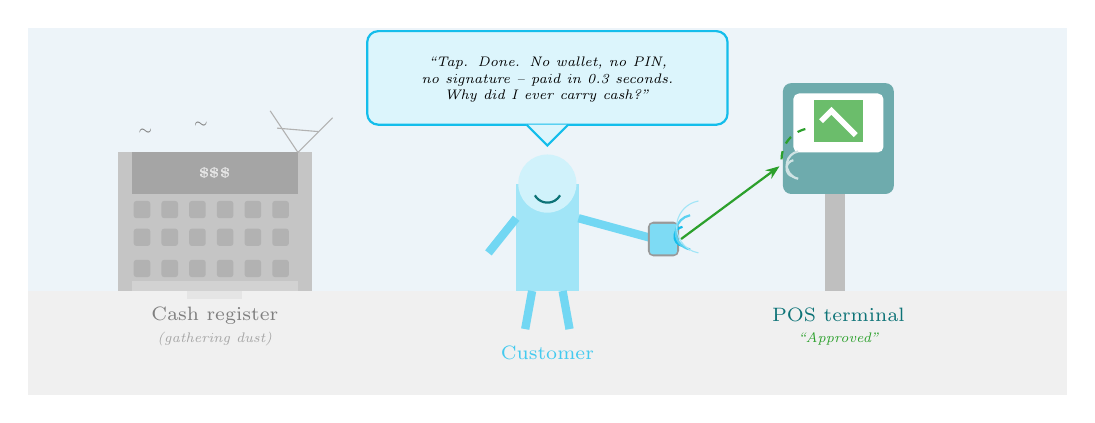
\begin{tikzpicture}[scale=0.88]

  % ---- Floor / background ------------------------------------
  \fill[mlgray!12] (-7.5,-1.5) rectangle (7.5,0.0);
  \fill[mlblue!8]  (-7.5, 0.0) rectangle (7.5,3.8);

  % ============================================================
  %  LEFT SIDE: dusty cash register
  % ============================================================
  % Cabinet
  \fill[mlgray!45] (-6.2,0.0) rectangle (-3.4,2.0);
  % Display
  \fill[mlgray!70] (-6.0,1.4) rectangle (-3.6,2.0);
  \node[font=\tiny\bfseries,text=mlgray!20] at (-4.8,1.7) {\$\$\$};
  % Key grid
  \foreach \x in {-5.85,-5.45,-5.05,-4.65,-4.25,-3.85}{
    \foreach \y in {0.2,0.65,1.05}{
      \fill[mlgray!60,rounded corners=1pt]
        (\x-0.12,\y) rectangle (\x+0.12,\y+0.25);
    }
  }
  % Drawer
  \fill[mlgray!35] (-6.0,0.0) rectangle (-3.6,0.15);
  \fill[mlgray!20] (-5.2,-0.12) rectangle (-4.4,0.0);
  % Cobweb top-right corner
  \draw[mlgray!60,thin] (-3.6,2.0) -- (-4.0,2.6);
  \draw[mlgray!60,thin] (-3.6,2.0) -- (-3.1,2.5);
  \draw[mlgray!60,thin] (-3.9,2.35) -- (-3.3,2.3);
  % Dust puffs
  \node[font=\tiny,text=mlgray] at (-5.8,2.3) {$\sim$};
  \node[font=\tiny,text=mlgray] at (-5.0,2.4) {$\sim$};
  % Label
  \node[font=\scriptsize,text=mlgray] at (-4.8,-0.35) {Cash register};
  \node[font=\tiny\itshape,text=mlgray!70] at (-4.8,-0.70) {(gathering dust)};

  % ============================================================
  %  CENTRE: Customer tapping phone
  % ============================================================
  % Body
  \fill[mlcyan!40] (-0.45,0.0) rectangle (0.45,1.55);
  % Head
  \fill[mlcyan!20] (0.0,1.55) circle (0.42);
  % Smile
  \draw[mlteal,thick] (-0.18,1.38) arc(210:330:0.21);
  % Right arm extended toward reader
  \draw[mlcyan!60,line width=3pt] (0.45,1.05) -- (1.55,0.75);
  % Phone in hand
  \fill[mlgray!80,rounded corners=2pt] (1.45,0.50) rectangle (1.90,1.00);
  \fill[mlcyan!55,rounded corners=1pt] (1.48,0.53) rectangle (1.87,0.97);
  % NFC wave from phone
  \draw[mlcyan,thick] (1.95,0.65) arc(260:100:0.14);
  \draw[mlcyan!70,thick] (2.06,0.60) arc(260:100:0.25);
  \draw[mlcyan!40,thin]  (2.18,0.55) arc(260:100:0.38);
  % Left arm down
  \draw[mlcyan!60,line width=3pt] (-0.45,1.05) -- (-0.85,0.55);
  % Legs
  \draw[mlcyan!60,line width=3pt] (-0.22,0.0) -- (-0.32,-0.55);
  \draw[mlcyan!60,line width=3pt] ( 0.22,0.0) -- ( 0.32,-0.55);
  \node[font=\scriptsize,text=mlcyan!80] at (0.0,-0.90) {Customer};

  % Speech bubble
  \fill[mlcyan!15,rounded corners=4pt] (-2.6,2.4) rectangle (2.6,3.75);
  \draw[mlcyan,thick,rounded corners=4pt] (-2.6,2.4) rectangle (2.6,3.75);
  \fill[mlcyan!15] (-0.3,2.4) -- (0.0,2.10) -- (0.3,2.4) -- cycle;
  \draw[mlcyan,thick] (-0.3,2.4) -- (0.0,2.10) -- (0.3,2.4);
  \node[font=\tiny,text width=4.8cm,align=center] at (0.0,3.05)
    {\textit{``Tap. Done. No wallet, no PIN,}\\
     \textit{no signature -- paid in 0.3 seconds.}\\
     \textit{Why did I ever carry cash?''}};

  % ============================================================
  %  RIGHT SIDE: POS terminal / card reader
  % ============================================================
  % Stand
  \fill[mlgray!50] (4.0,0.0) rectangle (4.3,1.4);
  % Terminal body
  \fill[mlteal!60,rounded corners=3pt] (3.4,1.4) rectangle (5.0,3.0);
  % Screen
  \fill[white,rounded corners=2pt] (3.55,2.0) rectangle (4.85,2.85);
  % Tick / approved message
  \fill[mlgreen!70] (3.85,2.15) rectangle (4.55,2.75);
  \draw[white,line width=2pt] (3.95,2.45) -- (4.10,2.60) -- (4.45,2.25);
  % Contactless symbol on terminal
  \draw[mlteal!20,thick] (3.55,1.65) arc(260:100:0.12);
  \draw[mlteal!20,thick] (3.62,1.62) arc(260:100:0.20);
  % NFC arc (receiving)
  \draw[mlgreen,thick,dashed] (3.38,1.9) arc(180:90:0.45);
  % Label
  \node[font=\scriptsize,text=mlteal] at (4.2,-0.35) {POS terminal};
  \node[font=\tiny\itshape,text=mlgreen] at (4.2,-0.70) {``Approved''};

  % Arrow: phone to terminal
  \draw[mlgreen,-{Stealth[length=5pt]},thick]
    (1.93,0.75) -- (3.35,1.80);

\end{tikzpicture}
\end{center}
\bottomnote{Slide 1/10 --- WHY | Global card-present transactions exceeded 400 billion in 2023 (illustrative). The shift from cash to tap took less than a decade.}
\end{frame}

% ============================================================
%  FRAME 2 -- FEEL: Text prompt ("Check your last 10 transactions")
% ============================================================
\begin{frame}{A Moment of Reflection: Your Last 10 Transactions}

\vspace{0.2em}
\begin{block}{The Payment Mix You Actually Use}
\small Payments are invisible until they fail. Before we analyse systems, let us look at your own behaviour as the data point.
\end{block}

\vspace{0.3em}
\small Open your banking or payments app and review your last 10 transactions. For each one, note:

\vspace{0.15em}
\begin{columns}[T]
\begin{column}{0.48\textwidth}
\begin{itemize}\small
  \item[\textcolor{mlteal}{\textbullet}] \textbf{Channel:} card, mobile wallet, bank transfer, cash?
  \item[\textcolor{mlteal}{\textbullet}] \textbf{Speed:} instant, same-day, or multi-day?
  \item[\textcolor{mlteal}{\textbullet}] \textbf{Visibility:} did you see any fees charged to you?
\end{itemize}
\end{column}
\begin{column}{0.48\textwidth}
\begin{itemize}\small
  \item[\textcolor{mlcyan}{\textbullet}] \textbf{Network:} Visa, Mastercard, domestic scheme, crypto?
  \item[\textcolor{mlcyan}{\textbullet}] \textbf{Consent:} one-click, biometric, PIN, or contactless?
  \item[\textcolor{mlcyan}{\textbullet}] \textbf{Cross-border:} same currency or FX conversion?
\end{itemize}
\end{column}
\end{columns}

\vspace{0.3em}
\begin{exampleblock}{Quick Tally}
\small How many of your 10 transactions were \textbf{card-based}? How many were \textbf{instant bank transfers}? Is there a single one that used \textbf{crypto}? What does your personal mix reveal about payment adoption in your country?
\end{exampleblock}

\bottomnote{Slide 2/10 --- FEEL | Your payment mix is shaped by regulation, merchant acceptance, and habit -- all forces this lecture will unpack.}
\end{frame}

% ============================================================
%  FRAME 3 -- WHAT: Table -- payment types comparison
%                           (cash, card, mobile, crypto)
% ============================================================
\begin{frame}{What Are the Payment Types? A Comparative Map}

\vspace{0.1em}
\begin{center}
\scriptsize
\begin{tabular}{@{}p{2.2cm}p{2.6cm}p{2.6cm}p{2.6cm}p{2.6cm}@{}}
\toprule
\textbf{Dimension} & \textbf{Cash} & \textbf{Card (Debit/Credit)} & \textbf{Mobile Wallet} & \textbf{Crypto / Stablecoin} \\
\midrule
\textbf{Settlement} & Instant, final & 1--3 business days & Varies (card rail or bank) & Seconds to hours \\[2pt]
\textbf{Reversibility} & \textcolor{mlred}{\textbf{None}} & \textcolor{mlgreen}{\textbf{Chargeback}} & \textcolor{mlorange}{\textbf{Partial}} & \textcolor{mlred}{\textbf{None (on-chain)}} \\[2pt]
\textbf{Anonymity} & \textcolor{mlgreen}{\textbf{High}} & \textcolor{mlred}{\textbf{Low}} & \textcolor{mlred}{\textbf{Low}} & \textcolor{mlorange}{\textbf{Pseudonymous}} \\[2pt]
\textbf{Merchant fee} & Zero & 1.5\%--3.5\% & 1\%--2.5\% & \textless{}1\% (varies) \\[2pt]
\textbf{FX / cross-border} & Manual exchange & 1\%--3\% surcharge & Platform-dependent & Low \emph{but volatile} \\[2pt]
\textbf{Consumer protection} & \textcolor{mlred}{\textbf{None}} & \textcolor{mlgreen}{\textbf{Strong (PSD2/Reg E)}} & \textcolor{mlorange}{\textbf{Moderate}} & \textcolor{mlred}{\textbf{Minimal}} \\[2pt]
\textbf{Infrastructure needed} & Physical cash & POS terminal, network & Smartphone + internet & Wallet + node access \\[2pt]
\textbf{Primary user pain} & Loss / theft & Fraud; slow settlement & Acceptance gaps & Volatility; complexity \\
\bottomrule
\end{tabular}
\end{center}

\vspace{0.1em}
\begin{block}{No Single Winner}
\scriptsize Each type trades off speed, cost, protection, and anonymity differently. Market share reflects regulation and merchant incentives, not consumer preference alone.
\end{block}

\bottomnote{Slide 3/10 --- WHAT | All fees and settlement times are illustrative. Real figures vary by country, scheme, and acquirer contract.}
\end{frame}

% ============================================================
%  FRAME 4 -- CASE: TikZ diagram -- four-party payment model
%                   (issuer, acquirer, network, merchant)
% ============================================================
\begin{frame}{The Four-Party Model: How One Card Tap Involves Four Entities}
\begin{center}
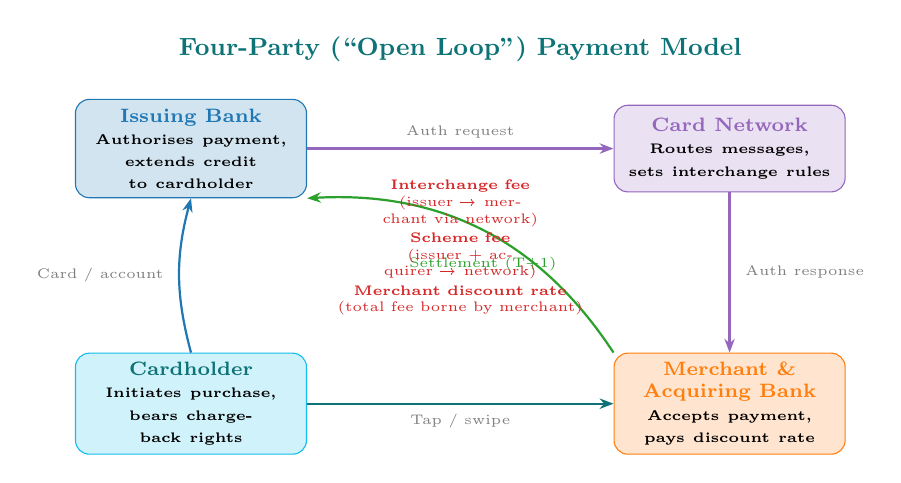
\begin{tikzpicture}[scale=0.90,
  box/.style={rectangle,rounded corners=5pt,minimum width=2.8cm,
              minimum height=1.1cm,font=\scriptsize\bfseries,
              text centered,text width=2.7cm},
  arr/.style={-{Stealth[length=5pt]},thick},
  lbl/.style={font=\tiny,text=mlgray,midway}
]

  % ---- Four nodes in a square layout -------------------------
  % Top-left: Cardholder / Issuing Bank
  \node[box,fill=mlblue!20,draw=mlblue] (issuer) at (-3.8, 1.8)
    {\textcolor{mlblue}{Issuing Bank}\\[2pt]
     \tiny Authorises payment,\\ extends credit to cardholder};

  % Top-right: Card Network
  \node[box,fill=mlpurple!20,draw=mlpurple] (network) at (3.8, 1.8)
    {\textcolor{mlpurple}{Card Network}\\[2pt]
     \tiny Routes messages,\\ sets interchange rules};

  % Bottom-left: Cardholder
  \node[box,fill=mlcyan!20,draw=mlcyan] (customer) at (-3.8,-1.8)
    {\textcolor{mlteal}{Cardholder}\\[2pt]
     \tiny Initiates purchase,\\ bears chargeback rights};

  % Bottom-right: Merchant + Acquirer
  \node[box,fill=mlorange!20,draw=mlorange] (acquirer) at (3.8,-1.8)
    {\textcolor{mlorange}{Merchant \&\\ Acquiring Bank}\\[2pt]
     \tiny Accepts payment,\\ pays discount rate};

  % ---- Arrows ------------------------------------------------
  % 1. Customer to Issuer (cardholder relationship)
  \draw[arr,mlblue,bend left=15]
    (customer.north) to node[lbl,left,xshift=-2pt]{Card / account} (issuer.south);

  % 2. Issuer to Network (authorisation request)
  \draw[arr,mlpurple]
    (issuer.east) to node[lbl,above]{Auth request} (network.west);

  % 3. Network to Acquirer (auth response)
  \draw[arr,mlpurple]
    (network.south) to node[lbl,right,xshift=2pt]{Auth response} (acquirer.north);

  % 4. Customer to Merchant (physical/digital payment)
  \draw[arr,mlteal]
    (customer.east) to node[lbl,below]{Tap / swipe} (acquirer.west);

  % 5. Acquirer to Issuer (clearing & settlement)
  \draw[arr,mlgreen,bend right=30]
    (acquirer.north west) to
    node[lbl,below,xshift=0pt,yshift=-6pt]{\textcolor{mlgreen}{Settlement (T+1)}}
    (issuer.south east);

  % ---- Fee labels --------------------------------------------
  \node[font=\tiny,text=mlred,align=center,text width=3.2cm]
    at (0, 0.4)
    {\textbf{Interchange fee}\\(issuer \textrightarrow{} merchant via network)\\[1pt]
     \textbf{Scheme fee}\\(issuer + acquirer \textrightarrow{} network)\\[1pt]
     \textbf{Merchant discount rate}\\(total fee borne by merchant)};

  % ---- Title label -------------------------------------------
  \node[font=\small\bfseries,text=mlteal] at (0, 3.2)
    {Four-Party (``Open Loop'') Payment Model};

\end{tikzpicture}
\end{center}
\bottomnote{Slide 4/10 --- CASE | Three-party schemes (e.g., Amex) collapse issuer and acquirer into one entity. Four-party schemes (Visa, Mastercard) separate them, enabling universal acceptance.}
\end{frame}

% ============================================================
%  FRAME 5 -- HOW: TikZ flow -- authorization -> clearing
%                               -> settlement lifecycle
% ============================================================
\begin{frame}{How a Payment Moves: Authorisation, Clearing, Settlement}
\begin{center}
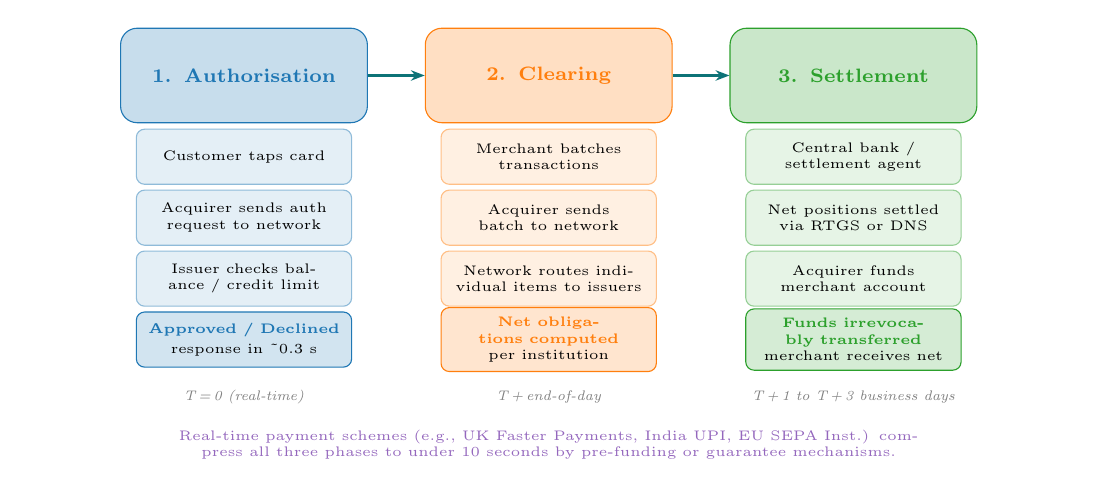
\begin{tikzpicture}[scale=0.86,
  phase/.style={rectangle,rounded corners=6pt,minimum width=3.0cm,
                minimum height=1.2cm,font=\scriptsize\bfseries,
                text centered,text width=2.9cm},
  stepbox/.style={rectangle,rounded corners=3pt,minimum width=2.6cm,
               minimum height=0.7cm,font=\tiny,
               text centered,text width=2.5cm},
  arr/.style={-{Stealth[length=5pt]},thick,mlteal},
  time/.style={font=\tiny\itshape,text=mlgray}
]

  % ---- Phase headers (top row) --------------------------------
  \node[phase,fill=mlblue!25,draw=mlblue]    (A) at (-4.5, 2.2)
    {\textcolor{mlblue}{1. Authorisation}};
  \node[phase,fill=mlorange!25,draw=mlorange] (B) at (0.0, 2.2)
    {\textcolor{mlorange}{2. Clearing}};
  \node[phase,fill=mlgreen!25,draw=mlgreen]  (C) at (4.5, 2.2)
    {\textcolor{mlgreen}{3. Settlement}};

  % Arrows between phases
  \draw[arr] (A.east) -- (B.west);
  \draw[arr] (B.east) -- (C.west);

  % ---- Step boxes under each phase ---------------------------
  % Authorisation steps
  \node[stepbox,fill=mlblue!12,draw=mlblue!50]  at (-4.5, 1.0)
    {Customer taps card};
  \node[stepbox,fill=mlblue!12,draw=mlblue!50]  at (-4.5, 0.1)
    {Acquirer sends auth request to network};
  \node[stepbox,fill=mlblue!12,draw=mlblue!50]  at (-4.5,-0.8)
    {Issuer checks balance / credit limit};
  \node[stepbox,fill=mlblue!20,draw=mlblue]     at (-4.5,-1.7)
    {\textcolor{mlblue}{\textbf{Approved / Declined}}\\[1pt]response in \textasciitilde{}0.3 s};

  \node[time] at (-4.5,-2.55) {T\,=\,0 (real-time)};

  % Clearing steps
  \node[stepbox,fill=mlorange!12,draw=mlorange!50] at (0.0, 1.0)
    {Merchant batches transactions};
  \node[stepbox,fill=mlorange!12,draw=mlorange!50] at (0.0, 0.1)
    {Acquirer sends batch to network};
  \node[stepbox,fill=mlorange!12,draw=mlorange!50] at (0.0,-0.8)
    {Network routes individual items to issuers};
  \node[stepbox,fill=mlorange!20,draw=mlorange]    at (0.0,-1.7)
    {\textcolor{mlorange}{\textbf{Net obligations computed}}\\per institution};

  \node[time] at (0.0,-2.55) {T\,+\,end-of-day};

  % Settlement steps
  \node[stepbox,fill=mlgreen!12,draw=mlgreen!50] at (4.5, 1.0)
    {Central bank / settlement agent};
  \node[stepbox,fill=mlgreen!12,draw=mlgreen!50] at (4.5, 0.1)
    {Net positions settled via RTGS or DNS};
  \node[stepbox,fill=mlgreen!12,draw=mlgreen!50] at (4.5,-0.8)
    {Acquirer funds merchant account};
  \node[stepbox,fill=mlgreen!20,draw=mlgreen]    at (4.5,-1.7)
    {\textcolor{mlgreen}{\textbf{Funds irrevocably transferred}}\\merchant receives net};

  \node[time] at (4.5,-2.55) {T\,+\,1 to T\,+\,3 business days};

  % ---- Bottom note on faster rails ---------------------------
  \node[font=\tiny,text=mlpurple,align=center,text width=13cm]
    at (0,-3.25)
    {Real-time payment schemes (e.g., UK Faster Payments, India UPI, EU SEPA Inst.)
     compress all three phases to under 10 seconds by pre-funding or guarantee mechanisms.};

\end{tikzpicture}
\end{center}
\bottomnote{Slide 5/10 --- HOW | The gap between authorisation (instant) and settlement (days) is where fraud, float, and counterparty risk live.}
\end{frame}

% ============================================================
%  FRAME 6 -- RISK: TikZ comic -- merchant looking at fee
%                                  breakdown statement
% ============================================================
\begin{frame}{The Hidden Cost: A Merchant Reads the Fee Statement}
\begin{columns}[T]
\begin{column}{0.50\textwidth}
\vspace{0.2em}
\begin{center}
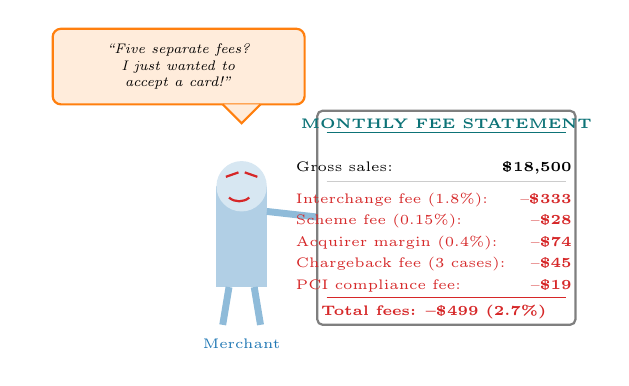
\begin{tikzpicture}[scale=0.80]

  % ---- Merchant figure (left) --------------------------------
  % Body
  \fill[mlblue!35] (-0.9,-0.6) rectangle (-0.1,1.0);
  % Head
  \fill[mlblue!18] (-0.5,1.0) circle (0.40);
  % Furrowed brow
  \draw[mlred,thick] (-0.75,1.15) -- (-0.55,1.22);
  \draw[mlred,thick] (-0.45,1.22) -- (-0.25,1.15);
  % Frown
  \draw[mlred,thick] (-0.7,0.82) arc(230:310:0.25);
  % Arm toward statement
  \draw[mlblue!50,line width=2.5pt] (-0.1,0.6) -- (0.8,0.5);
  % Legs
  \draw[mlblue!50,line width=2.5pt] (-0.7,-0.6) -- (-0.8,-1.2);
  \draw[mlblue!50,line width=2.5pt] (-0.3,-0.6) -- (-0.2,-1.2);
  \node[font=\tiny,text=mlblue] at (-0.5,-1.5) {Merchant};

  % ---- Fee statement (right) ---------------------------------
  % Paper
  \fill[white,draw=mlgray,thick,rounded corners=2pt]
    (0.7,-1.2) rectangle (4.8,2.2);
  % Heading
  \node[font=\tiny\bfseries,text=mlteal] at (2.75,2.0) {MONTHLY FEE STATEMENT};
  \draw[mlteal,thin] (0.85,1.85) -- (4.65,1.85);

  % Line items
  \node[font=\tiny,align=left,text width=3.5cm] at (2.55,1.3)
    {Gross sales: \hfill \textbf{\$18,500}};
  \draw[mlgray!40,thin] (0.85,1.07) -- (4.65,1.07);

  \node[font=\tiny,align=left,text width=3.5cm,text=mlred] at (2.55,0.78)
    {Interchange fee (1.8\%): \hfill --\textbf{\$333}};
  \node[font=\tiny,align=left,text width=3.5cm,text=mlred] at (2.55,0.44)
    {Scheme fee (0.15\%): \hfill --\textbf{\$28}};
  \node[font=\tiny,align=left,text width=3.5cm,text=mlred] at (2.55,0.10)
    {Acquirer margin (0.4\%): \hfill --\textbf{\$74}};
  \node[font=\tiny,align=left,text width=3.5cm,text=mlred] at (2.55,-0.24)
    {Chargeback fee (3 cases): \hfill --\textbf{\$45}};
  \node[font=\tiny,align=left,text width=3.5cm,text=mlred] at (2.55,-0.58)
    {PCI compliance fee: \hfill --\textbf{\$19}};
  \draw[mlred,thin] (0.85,-0.76) -- (4.65,-0.76);

  \node[font=\tiny\bfseries,text=mlred] at (2.55,-1.0)
    {Total fees: \hfill --\textbf{\$499} (2.7\%)};

  % Merchant speech bubble
  \fill[mlorange!15,rounded corners=3pt] (-3.5,2.3) rectangle (0.5,3.5);
  \draw[mlorange,thick,rounded corners=3pt] (-3.5,2.3) rectangle (0.5,3.5);
  \fill[mlorange!15] (-0.8,2.3) -- (-0.5,2.0) -- (-0.2,2.3) -- cycle;
  \draw[mlorange,thick] (-0.8,2.3) -- (-0.5,2.0) -- (-0.2,2.3);
  \node[font=\tiny,text width=3.6cm,align=center] at (-1.5,2.9)
    {\textit{``Five separate fees?}\\
     \textit{I just wanted to}\\
     \textit{accept a card!''}};

\end{tikzpicture}
\end{center}
\end{column}
\begin{column}{0.46\textwidth}
\vspace{0.2em}
\begin{alertblock}{Where the Risk Concentrates}
\scriptsize
\textbf{Interchange opacity:} Merchants rarely know the exact interchange rate per card type before accepting.\\[3pt]
\textbf{Chargeback liability:} Card-not-present fraud shifts 100\% of loss to merchant.\\[3pt]
\textbf{Scheme rule changes:} Networks unilaterally adjust fee structures, sometimes with 30-day notice.\\[3pt]
\textbf{Lock-in:} Switching acquirers requires hardware changes, re-certification, and new contracts.
\end{alertblock}
\vspace{0.2em}
\begin{block}{Merchant Responses}
\scriptsize
Surcharging (where legal), steering to lower-cost methods (debit over credit, ACH), or adopting alternative schemes (local RTP rails, crypto at POS for lower fees).
\end{block}
\end{column}
\end{columns}
\bottomnote{Slide 6/10 --- RISK | All figures are illustrative. Actual interchange varies by card type, merchant category code (MCC), and acquiring contract.}
\end{frame}

% ============================================================
%  FRAME 7 -- WHERE: pgfplots bar chart --
%             real-time payment adoption by country (illustrative)
% ============================================================
\begin{frame}{Where Is Real-Time Payments Growing? Illustrative Adoption Snapshot}
\vspace{0.05em}
\begin{center}
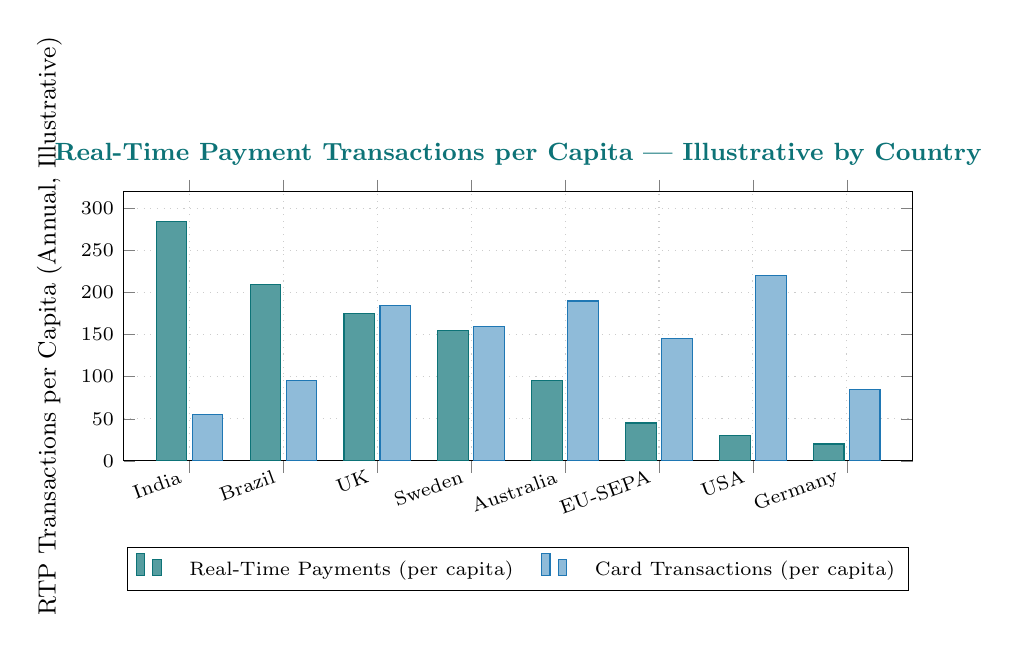
\begin{tikzpicture}
\begin{axis}[
  width=11.6cm, height=5.0cm,
  ybar=2pt,
  bar width=11pt,
  enlarge x limits=0.10,
  ylabel={\small RTP Transactions per Capita (Annual, Illustrative)},
  ylabel style={font=\scriptsize},
  symbolic x coords={India, Brazil, UK, Sweden, Australia, EU-SEPA, USA, Germany},
  xtick=data,
  xticklabel style={font=\scriptsize, rotate=20, anchor=east},
  ymin=0, ymax=320,
  ytick={0,50,100,150,200,250,300},
  yticklabel style={font=\scriptsize},
  legend style={font=\scriptsize, at={(0.5,-0.32)}, anchor=north,
                legend columns=2, column sep=8pt},
  legend cell align=left,
  grid=major,
  grid style={dotted,mlgray!40},
  title={\small\bfseries\textcolor{mlteal}{Real-Time Payment Transactions per Capita --- Illustrative by Country}},
  title style={font=\small},
  clip=false,
]

% RTP transactions per capita (illustrative)
\addplot[fill=mlteal!70,draw=mlteal] coordinates {
  (India,    285)
  (Brazil,   210)
  (UK,       175)
  (Sweden,   155)
  (Australia, 95)
  (EU-SEPA,   45)
  (USA,       30)
  (Germany,   20)
};

% Cards per capita for comparison (illustrative)
\addplot[fill=mlblue!50,draw=mlblue] coordinates {
  (India,     55)
  (Brazil,    95)
  (UK,       185)
  (Sweden,   160)
  (Australia,190)
  (EU-SEPA,  145)
  (USA,      220)
  (Germany,   85)
};

\legend{Real-Time Payments (per capita), Card Transactions (per capita)}
\end{axis}
\end{tikzpicture}
\end{center}
\vspace{-0.4em}
{\tiny\textcolor{mlgray}{All figures illustrative and indicative of relative scale only. Based on publicly reported trends from ACI Worldwide, BIS, and central bank reports through 2023.}}
\bottomnote{Slide 7/10 --- WHERE | India's UPI and Brazil's Pix achieved mass adoption by mandating bank participation and offering zero-fee peer-to-peer transactions.}
\end{frame}

% ============================================================
%  FRAME 8 -- IMPACT: TikZ quadrant diagram --
%                     speed vs. cost of payment types
% ============================================================
\begin{frame}{Impact Map: Speed vs.\ Cost Across Payment Methods}
\vspace{0.1em}
\begin{center}
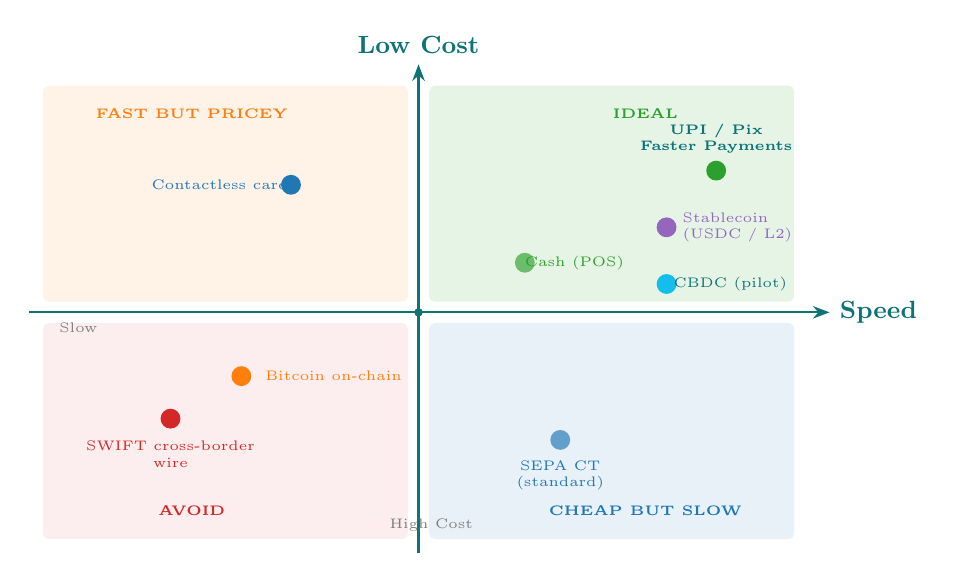
\begin{tikzpicture}[scale=0.90]

  % ---- Quadrant shading --------------------------------------
  % Top-right: Fast + Cheap (ideal)
  \fill[mlgreen!12,rounded corners=2pt] (0.15,0.15) rectangle (5.3,3.2);
  % Top-left: Fast + Expensive
  \fill[mlorange!10,rounded corners=2pt] (-5.3,0.15) rectangle (-0.15,3.2);
  % Bottom-right: Slow + Cheap
  \fill[mlblue!10,rounded corners=2pt] (0.15,-3.2) rectangle (5.3,-0.15);
  % Bottom-left: Slow + Expensive (avoid)
  \fill[mlred!8,rounded corners=2pt] (-5.3,-3.2) rectangle (-0.15,-0.15);

  % ---- Axes --------------------------------------------------
  \draw[-{Stealth[length=6pt]},mlteal,thick] (-5.5,0) -- (5.8,0)
    node[right,font=\small\bfseries,text=mlteal] {Speed};
  \draw[-{Stealth[length=6pt]},mlteal,thick] (0,-3.4) -- (0,3.5)
    node[above,font=\small\bfseries,text=mlteal] {Low Cost};

  % Axis end labels
  \node[font=\tiny,text=mlgray] at (-4.8,-0.22) {Slow};
  \node[font=\tiny,text=mlgray] at ( 0.18,-3.0) {High Cost};

  % ---- Quadrant labels --------------------------------------
  \node[font=\tiny\bfseries,text=mlgreen]   at ( 3.2, 2.8) {IDEAL};
  \node[font=\tiny\bfseries,text=mlorange]  at (-3.2, 2.8) {FAST BUT PRICEY};
  \node[font=\tiny\bfseries,text=mlblue]    at ( 3.2,-2.8) {CHEAP BUT SLOW};
  \node[font=\tiny\bfseries,text=mlred]     at (-3.2,-2.8) {AVOID};

  % ---- Payment method dots -----------------------------------
  % UPI / Faster Payments (fast, near-zero cost)
  \fill[mlgreen]   (4.2, 2.0) circle (0.14);
  \node[font=\tiny\bfseries,text=mlteal,align=center] at (4.2,2.45)
    {UPI / Pix\\Faster Payments};

  % Stablecoins on fast L1 (fast, low cost)
  \fill[mlpurple]  (3.5, 1.2) circle (0.14);
  \node[font=\tiny,text=mlpurple,align=left] at (4.5,1.2)
    {Stablecoin\\(USDC / L2)};

  % Contactless card (fast, moderate cost)
  \fill[mlblue]    (-1.8, 1.8) circle (0.14);
  \node[font=\tiny,text=mlblue]  at (-2.8,1.8) {Contactless card};

  % Wire transfer SWIFT (slow, expensive)
  \fill[mlred]     (-3.5,-1.5) circle (0.14);
  \node[font=\tiny,text=mlred,align=center] at (-3.5,-2.0)
    {SWIFT cross-border\\wire};

  % Bitcoin on-chain (slow, high fee in congestion)
  \fill[mlorange]  (-2.5,-0.9) circle (0.14);
  \node[font=\tiny,text=mlorange,align=left] at (-1.2,-0.9)
    {Bitcoin on-chain};

  % SEPA Credit Transfer (slow, low cost)
  \fill[mlblue!70] (2.0,-1.8) circle (0.14);
  \node[font=\tiny,text=mlblue,align=center] at (2.0,-2.3)
    {SEPA CT\\(standard)};

  % Cash (instant at POS, zero direct cost)
  \fill[mlgreen!70] (1.5, 0.7) circle (0.14);
  \node[font=\tiny,text=mlgreen,align=left] at (2.2,0.7)
    {Cash (POS)};

  % CBDC (pilot) -- fast, low cost, uncertain
  \fill[mlcyan]    (3.5, 0.4) circle (0.14);
  \node[font=\tiny,text=mlteal,align=left] at (4.4,0.4)
    {CBDC (pilot)};

  % Origin
  \fill[mlteal] (0,0) circle (0.06);

\end{tikzpicture}
\end{center}
\bottomnote{Slide 8/10 --- IMPACT | Positions are illustrative. Real-time rail design is converging toward the top-right corner; legacy cross-border wires remain stranded in the bottom-left.}
\end{frame}

% ============================================================
%  FRAME 9 -- SO WHAT: Evaluation checklist --
%             5 questions for any payment system
% ============================================================
\begin{frame}{So What? Five Questions to Evaluate Any Payment System}

\vspace{0.3em}
\begin{columns}[T]
\begin{column}{0.62\textwidth}

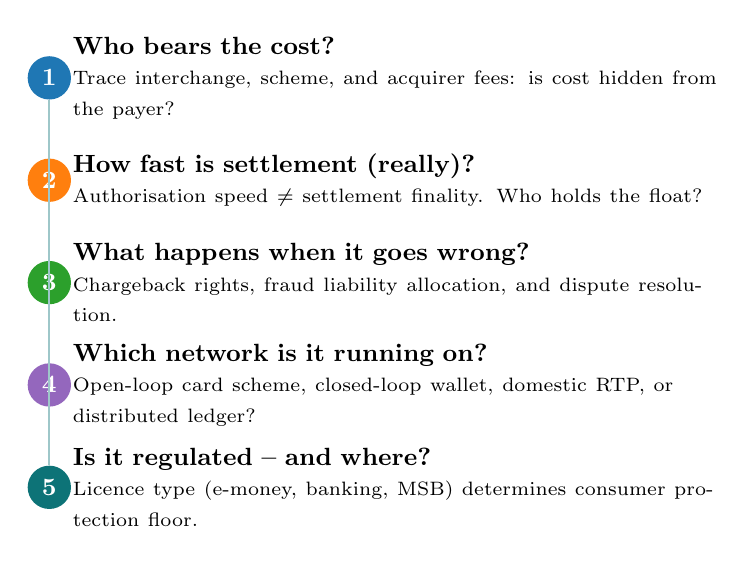
\begin{tikzpicture}[
  chk/.style={circle,minimum size=0.55cm,font=\small\bfseries,
              inner sep=0pt,text=white},
  lbl/.style={font=\small,text width=8.2cm,align=left}
]

% ---- Row 1 --------------------------------------------------
\node[chk,fill=mlblue]    (c1) at (0, 0)   {1};
\node[lbl] at (4.4, 0)
  {\textbf{Who bears the cost?}\\
   {\scriptsize Trace interchange, scheme, and acquirer fees: is cost hidden from the payer?}};

% ---- Row 2 --------------------------------------------------
\node[chk,fill=mlorange]  (c2) at (0,-1.3) {2};
\node[lbl] at (4.4,-1.3)
  {\textbf{How fast is settlement (really)?}\\
   {\scriptsize Authorisation speed $\neq$ settlement finality. Who holds the float?}};

% ---- Row 3 --------------------------------------------------
\node[chk,fill=mlgreen]   (c3) at (0,-2.6) {3};
\node[lbl] at (4.4,-2.6)
  {\textbf{What happens when it goes wrong?}\\
   {\scriptsize Chargeback rights, fraud liability allocation, and dispute resolution.}};

% ---- Row 4 --------------------------------------------------
\node[chk,fill=mlpurple]  (c4) at (0,-3.9) {4};
\node[lbl] at (4.4,-3.9)
  {\textbf{Which network is it running on?}\\
   {\scriptsize Open-loop card scheme, closed-loop wallet, domestic RTP, or distributed ledger?}};

% ---- Row 5 --------------------------------------------------
\node[chk,fill=mlteal]    (c5) at (0,-5.2) {5};
\node[lbl] at (4.4,-5.2)
  {\textbf{Is it regulated -- and where?}\\
   {\scriptsize Licence type (e-money, banking, MSB) determines consumer protection floor.}};

% Vertical connector line
\draw[mlteal!40,thick] (0,-0.28) -- (0,-4.92);

\end{tikzpicture}

\end{column}
\begin{column}{0.34\textwidth}
\vspace{0.2em}
\begin{block}{When to Use This}
\scriptsize
\begin{itemize}
  \item Assessing a payments startup pitch
  \item Evaluating a PSP for your business
  \item Writing a fintech regulatory memo
  \item Completing the Day-5 Payments Workshop exercise
\end{itemize}
\end{block}
\vspace{0.2em}
\begin{exampleblock}{Worked Example}
\scriptsize
\textbf{UPI (India, 2016--)}\\
Cost bearer: government subsidy\\
Settlement: near-instant (IMPS)\\
Wrong: NPCI dispute framework\\
Network: domestic RTP rail\\
Regulation: RBI licensed, NPCI governed
\end{exampleblock}
\end{column}
\end{columns}

\bottomnote{Slide 9/10 --- SO WHAT | These five questions apply equally to cash, cards, mobile wallets, real-time rails, and crypto payment layers.}
\end{frame}

% ============================================================
%  FRAME 10 -- ACT: Activity prompt + next lecture preview
%                   (L04: Fintech Security and Regulation -- RegTech)
% ============================================================
\begin{frame}{Act: Map a Payment Journey End to End}

\begin{columns}[T]
\begin{column}{0.56\textwidth}
\begin{block}{Your Task (15 Minutes)}
\scriptsize
Choose \textbf{one recent payment} you made (card, mobile, or transfer). Reconstruct the full lifecycle:
\begin{enumerate}\scriptsize
  \item \textbf{Authorisation:} Who approved it, in how long, using what check?
  \item \textbf{Clearing:} Which network carried the message? When was the batch sent?
  \item \textbf{Settlement:} When did funds actually move? Who received net cash?
  \item \textbf{Fees:} Estimate interchange + scheme + acquirer fees paid in total.
  \item \textbf{Five-question test:} Apply the checklist from Slide 9. Any weak points?
\end{enumerate}
\end{block}
\vspace{0.2em}
\begin{exampleblock}{Reflection Prompt}
\scriptsize
If you were the \textbf{merchant}, would you steer customers to a cheaper method? If you were the \textbf{regulator}, which fee layer would you cap first and why?
\end{exampleblock}
\end{column}
\begin{column}{0.40\textwidth}
\begin{exampleblock}{Discussion Starter}
\scriptsize
\begin{itemize}
  \item Real-time payment rails are ``free to users'' -- who actually funds them?
  \item Can crypto genuinely compete with Visa on cost \emph{and} consumer protection?
  \item Why did the US adopt real-time payments (FedNow) a decade after the UK?
\end{itemize}
\end{exampleblock}
\vspace{0.2em}
\begin{alertblock}{Next Lecture --- L04}
\scriptsize \textbf{Fintech Security and Regulation: RegTech}\\
From KYC to AML to algorithmic compliance: how technology is reshaping the regulatory frontier.\\[3pt]
\textit{Prepare: look up your bank's AML disclosure in its annual report.}
\end{alertblock}
\end{column}
\end{columns}

\bottomnote{Slide 10/10 --- ACT | Payments infrastructure is policy infrastructure. Every design choice -- speed, cost, reversibility -- is also a distributional choice about who bears risk.}
\end{frame}

% ============================================================
\end{document}
% ============================================================
